
\documentclass[11pt]{article}
  	\usepackage{ucs} 
	\usepackage[utf8x]{inputenc} % Включаем поддержку UTF8  
	\usepackage[russian]{babel}  % Включаем пакет для поддержки русского языка 
	\usepackage {mathtext}
	\usepackage{amsmath, amssymb}
	\usepackage{graphicx}
	\usepackage{listings}
	\usepackage{hyperref}
	\usepackage{revsymb}
	\usepackage{listings}
\lstset{language=[90]Fortran,
  basicstyle=\ttfamily,
  keywordstyle=\color{red},
  commentstyle=\color{green},
  morecomment=[l]{!\ }% Comment only with space after !
}
	\hypersetup{
    colorlinks=true,
    linkcolor=blue,
    filecolor=magenta,      
    urlcolor=cyan,
	}
	\urlstyle{same}
	\DeclareGraphicsExtensions{.pdf,.png,.jpg,.jpeg}

	\graphicspath{{pictures/}}
    \title{\textbf{Практическое исследование цепочки Гейзенберга S=1/2 \\ Часть III \\ -- \\ 
	Practical study of the Heisenberg chain S=1/2 \\ Part III}}
    \author{И.А.Юхновский}
    \date{ноябрь 2020}
    
\begin{document}

\maketitle
\thispagestyle{empty}
\section*{Аннотация}
Заключительная часть работы <<Практическое исследование цепочки Гейзенберга S = 1/2>> рассматривает вопросы запутанности для перехода от физического эксперимента к квантовым вычислениям. Рассматривается запутанность, индуцированная в частицах со спином 1/2 спиновой цепочкой в качестве теоретического обоснования актуальности проведения эксперимента по облучению одномерных магнетиков частицами ионизирующего излучения при нормальных условиях и сравнении результатов на цепочках ультра-холодных атомов. 


\section*{Abstract}
The final part of the work << Practical Investigation of the Heisenberg Chain S = 1/2 >> deals with entanglement issues for the transition from physical experiment to quantum computing. The entanglement induced in particles with a spin 1/2 by a spin chain is considered as a theoretical substantiation of the relevance of an experiment on irradiating one-dimensional magnets with ionizing radiation particles under normal conditions and comparing the results on chains of ultra-cold atoms

\tableofcontents{}

\section{Введение}
 В ~\cite{yi} в 2006 была установлена связь между запутанностью и критичностью спиновых цепочек на ультра-холодных атомах. Рассматривалась запутанность, которая разделяется между вспомогательными частицами, которые изолированы друг от друга, но связаны с одной и той же критической цепочкой со спином 1/2. Была сделана аналитическая оценка приведённой матрицы плотности и численно показана запутанность вспомогательных частиц вблизи критических точек спиновой цепочки. Была обнаружена, что запутанность, вызванная спиновой цепочкой, может достигать 1, и это может очень хорошо сигнализировать о критических точках цепочки. Представлены физическое понимание и экспериментальная реализация с захваченными ионами. Цель данной работы рассмотреть механизм запутанности на одномерных спиновых цепочках и подготовить теоретическое обоснование квантового эксперимента по облучению частицами ионизирующего излучения

\section{Запутанность}
йй

\section{Эксперимент Йи}
Квантовая запутанность лежит в основе разницы между квантовым и классическим многочастичным миром и может рассматриваться как полезный ресурс в различных задачах, таких как:
\begin{itemize} 
	\item криптография, 
	\item квантовые вычисления
	\item телепортация ~\cite{b1}, 
\end{itemize} 

Квантовые фазовые переходы ~\cite{2} - это переходы между квантовыми вычислениями. отдельные фазы квантовых систем многих тел, управляемые исключительно квантовыми флуктуациями. В последнее десятилетие были предприняты большие усилия, чтобы понять взаимосвязь между запутанностью и квантовыми фазовыми переходами 3–9. На самом деле, естественно связывать квантовый фазовый переход и запутанность, если за ними стоят корреляции. Разделяя эту точку зрения, можно ожидать, что запутанность, вызванная квантовой критической системой многих тел, даст впечатляющую сигнатуру квантовых критических точек для системы многих тел.

С другой стороны, мы обычно думаем об окружающей среде, окружающей квантовую систему, как об источнике декогеренции. Недавно исследователи начали изучать положительные эффекты ~\cite{b10,b11,b12,b13,b14,b15,b16,b17} окружающей среды, например, обработку информации, обусловленную окружающей средой, и запутанность, вызываемую окружающей средой. Эти исследования открывают новый путь к разработке механизмов предотвращения, минимизации или использования воздействия окружающей среды при обработке квантовой информации. Однако в этих работах окружающая среда моделировалась как набор независимых квантовых систем, то есть корреляций между частицами в окружающей среде. игнорировались. Интересный открытый вопрос заключается в том, может ли корреляция между частицами окружающей среды влиять на запутанность, индуцированную в двух частичной системе, которая с ней соединяется.

В этой статье мы покажем, как использовать запутанность во вспомогательных частицах, индуцированную квантовой критической системой многих тел, в качестве важного инструмента для выявления квантовых явлений в квантовой системе многих тел. Действительно, квантовые фазовые переходы сопровождаются качественным изменением характера классических корреляций, такие резкие изменения свойств основных состояний часто связаны с коллективностью и/или случайностью межчастичных взаимодействий, которые, возможно, отражаются в запутанности между системами, которые с ними связаны. Здесь мы принимаем систему спиновых цепочек, описываемую одномерной моделью спина 1/2XY как систему многих тел. Другая пара систем со спином 1/2, которые связаны со спиновой цепочкой, будет действовать как вспомогательные частицы. Мы видим, что спутанность вспомогательных частиц резко меняется в зависимости от близости квантового фазового перехода. Это изменение можно проследить до наличия коллективности в доминирующих связях вспомогательных частиц с цепочкой, а затем оно отражает критические свойства системы многих тел. Это наблюдение предлагает новый инструмент для изучения квантовых критических явлений, в частности, для более общих систем, для которых аналитические решения могут быть недоступны. Предлагается возможная реализация этой схемы с захваченными ионами. Он использует нерезонансные ионы, управляемые стоячими волнами, в ловушках ~\cite{b18,b19} для моделирования одномерной цепочки XY спина. Это предложение также могло быть реализовано с ультра-холодными атомами, наложенными на оптическую решётку ~cite{20}. Это делает исследование привлекательным для экспериментального тестирования.

Рассмотрим двудольную систему, состоящую из двух частиц со спином 1/2 $a$ и $b$, и квантовую систему многих тел, описываемую одномерной моделью со спином 1/2XY. Системный гамильтониан $H_S$ и гамильтониан $H_B$ цепи имеют вид


\begin{equation*}
H_S=\frac{\omega_a}{2}\sigma_a^Z+\frac{\omega_b}{2}\sigma_b^Z
\end{equation*}

\begin{equation}
H_B=-\sum\limits_{l=1}^N(\frac{1+\gamma}{2}\sigma_l^x\sigma_{l+1}^x
+ \frac{1-\gamma}{2}\sigma_l^y\sigma_{l+1}^y
+ \frac{\lambda}{2}\sigma_l^z
)
\label{eq_1}
\end{equation}

где N - число узлов, $\sigma_i^\alpha(\alpha=x,y,z)$ - матрицы Паули, $\gamma$- безразмерный параметр анизотропии. Для спиновой цепочки предполагается периодическое граничное условие $\sigma_{N + 1} = \sigma_1$. Предположим, что связь вспомогательных частиц в цепочку принимает вид

\begin{equation}
H_l=\sum\limits_{l=1}^N(g\sigma_a^z\sigma_l^z+h\sigma_b^z\sigma_l^z)
\label{eq_2}
\end{equation}

где $g$ и $h$ обозначают изменённые безразмерные константы связи. Ясно, что $[H_S, H_l] = 0$, что означает, что энергия вспомогательных частиц сохраняется, но когерентность может не сохраняться в зависимости от деталей связи системы и цепи. Это приводит к следующей форме оператора эволюции во времени $U(t)$ 

\begin{equation}
U(t)=\sum\limits_{i,j=0,1}U_{ij}(t)|ij\rangle\langle ij|
\label{eq_3}
\end{equation}

, где $|ij\rangle = |i\rangle_a \otimes |j\rangle_b$ и $|i\rangle_a(|i\rangle_b,i=0,1)$ представляет собственные состояния $\sigma_a^z(\sigma_b^z)$.

Легко показать что $U_{ij}(t)(i,j=0,1)$ удовлетворяет:

\begin{equation}
i\hbar\frac{\partial}{\partial t}U_{ij}(t)=H_{ij}U_{ij}(t)
\label{eq_4}
\end{equation}

где:

\begin{equation*}
H_{ij}=-\sum\limits_{l=1}^N(\frac{1+\gamma}{2}\sigma_l^x\sigma_{l+1}^x+\frac{1-\gamma}{2}\sigma_l^y\sigma_{l+1}^y+\frac{\Lambda_{ij}}{2}\sigma_l^z)
\end{equation*}

где:

\begin{equation*}
\Lambda_{ij}=\lambda+(-1)^{i+1}2g+(-1)^{j+1}2h,i,j=0,1
\end{equation*}

Если вспомогательные частицы изначально находятся в состоянии $|ij\rangle$, динамика и статистические свойства спиновой цепочки будут определяться величиной $H_ij$, которая принимает ту же форму что и  $H_B$ но с изменёнными значениями напряжённости поля $\Lambda_{ij}$. Гамильтониан $H_{ij}$ должен быть диагонализирован по стандартной процедуре ~\cite{b21} следующим образом:

\begin{equation*}
H_ij=\sum\limits_k\omega_{ij,k}(\eta_{ij,k}^†\eta_{ij,k}-\frac{1}{2})
\end{equation*}

,где $\eta_{ij,k}(\eta_{ij,k}^†)$ операторы аннигиляции фермионных мод с частотой:

\begin{equation*}
\omega_{ij,k}=\sqrt{\epsilon_{ij,k}^2+\gamma^2sin^2\frac{2\pi k}{N}}
\end{equation*}

,где:
 
\begin{equation*}
\epsilon_{ij,k}=(cos\frac{2\pi k}{N}-\Lambda_{ij}), k=-\frac{N}{2},-\frac{N}{2}+1, \dots , \frac{N}{2}-1
\end{equation*}
 
Фермионный оператор $\eta_{ij,k}$, k был определён преобразованием Боголюбова как:

\begin{equation*}
\eta_{ij,k}=d_kcos\frac{\Theta_{ij,k}}{2}-id_{-k}^†sin\frac{\Theta_{ij,k}}{2}
\end{equation*}

,где:

\begin{equation*}
d_k=\frac{1}{\sqrt{N}} \sum\limits_l a_l e^{\frac{-i2\pi lk}{N}}
\end{equation*}

а угол смещения $\Theta_{ij,k}$ был определён как

\begin{equation*}
cos\Theta_{ij,k}=\frac{\epsilon_{ij,k}}{\omega_{ij,k}}
\end{equation*}

Фермионные операторы $a_l$ были связаны со спиновыми операторами преобразованием Жордана-Вигнера через

\begin{equation*}
a_l=(\prod_{m<l}\sigma_m^z)(\sigma_l^x+i\sigma_l^y)/2
\end{equation*}

Операторы $\eta_{ij,k}$, параметризованные с помощью $i$ и $j$, явно не коммутируют друг с другом, это приводит к запутыванию во вспомогательных частицах, как будет показано ниже. Прежде чем перейти к вычислению приведённой матрицы плотности, мы обсудим диагонализацию $H_ij$. Для цепочки с периодическим граничным условием, т.е. $\sigma_1 = \sigma_N$, граничные члены:

\begin{equation*}
H_{bound} \sim [(a_N^†a_1+\gamma a_N a_1)+H.c.]e^{i\pi M}+1
\end{equation*}

необходимо принять во внимание ~\cite{b21,b22}. В этой статье мы будем работать с игнорированием момента указанного в ~\cite{b21}
M не является неизменным при преобразовании Боголюбова, однако его чётность или нечётность даёт ($e^{i\pi M}$, инвариантен):  

 Члены с $e^{i\pi M} = −1$ дают нулевой вклад в $\Gamma_{ij;mn}(t)$, потому что в этом случае граничные члены исчезают. 
 
 При $e^{i\pi M} = 1$ граничные члены изменяют порядок $1/N$ в $cos(\Theta_{ij,k}/2)$ и $sin(\Theta_{ij,k}/2)$. Поэтому они вносят поправки до порядка $1/N$ в $\Gamma_{ij;mn}(t)$, которыми можно безопасно пренебречь в пределе $N \rightarrow \infty$. Интуитивно, при $N \rightarrow \infty$ два случая открытой границы и циклической границы становятся одинаковыми, поэтому граничный эффект в этом смысле исчезнет.

Игнорируем потому, что мы заинтересованы в обнаружении связи между критичностью цепи и запутанностью во вспомогательных частицах.

Задав начальное состояние отделимости продукта общей системы:
\begin{equation*}
|\psi(0)\rangle = |\phi_a(0)\rangle \otimes |\phi_b(0)\rangle \otimes |\phi_B(0)\rangle
\end{equation*} 
 , мы можем получить приведённую матрицу плотности для вспомогательных частиц как

\begin{equation*}
\rho_{ab}(t)=Tr_B[U(t)|\psi(0)\rangle \langle \psi(0)|U^†(t)]
\end{equation*}
 
и его можно формально записать в виде:

\begin{equation*}
\rho_{ab}(t)=\sum\limits_{i,j;mn}\rho_{ij;mn}(t)|ij\rangle \langle mn|
\end{equation*}

Простой, но несколько утомительный расчёт показывает, что:
\begin{equation*}
\rho_{ij;mn}(t)=\rho_{ij;mn}(t=0)\Gamma_{ij;mn}(t)
\end{equation*}

,где:

\begin{equation}
\begin{gathered}
\Gamma_{ij;mn}(t)=\prod_k e^{(i/2)(\omega_{ij,k}-\omega_{mn,k})t}[\\
1-(1-e^{i\omega_{ij,k}t})sin^2\frac{\Theta_k-\Theta_{ij,k}}{2} \\
- (1-e^{-i\omega_{mn,k}t})sin^2\frac{\Theta_k-\Theta_{mn,k}}{2} \\
+ (1-e^{i\omega_{ij,k}t})(1-e^{i\omega_{mn,k}t}) \\
\times (sin\frac{\Theta_k-\Theta_{ij,k}}{2}sin\frac{\Theta_k-\Theta_{mn,k}}{2}
cos\frac{\Theta_{ij,k}-\Theta_{mn,k}}{2}
)
]
\end{gathered}
\label{eq_5}
\end{equation}

,где:
\begin{equation*}
cos \Theta_k = \frac{cos(2\pi k / N)-\lambda}
{\sqrt{[cos(2 \pi k / N) - \lambda]^2+\gamma^2 sin^2 (2\pi k / N)}}
\end{equation*}

Для получения этого результата предполагалось, что спиновая цепочка изначально находится в основном состоянии $H_B$. Обсуждения по формуле ~\ref{eq_5} в порядке.

Для $g=h$: $\Lambda_{ij}=\lambda$ и $j=1$ или $i=1$ и $j=0$.

Следовательно, $|01\rangle$ и $|10\rangle$ расширяют подпространство, свободное от декогеренции. Впоследствии запутанность состояний в этом подпространстве остаётся неизменной благодаря $\Gamma_{ij;mn}(t)=1$. Ситуация меняется, если $h \ne g$, где свободное от некогерентности подпространство не существует. Запутанность, разделяемая между вспомогательными частицами, эволюционирует со временем в соответствии с уравнением ~\ref{eq_5} в этой ситуации.

Используя эти выражения, мы переходим к изучению запутанности, разделяемой между вспомогательными частицами и состоянием ~\ref{eq_3}. Для конкретности в качестве начального состояния вспомогательных частиц выберем $|\phi_a(0) \rangle \otimes |\phi_b(0) = 1/\sqrt{2}(|0\rangle_a+|1\rangle_a) \otimes 1/\sqrt{2}(|0\rangle_b+|1\rangle_b)$, а спиновая цепочка предполагается находящейся в основном состоянии гамильтониана $H_B$. Запутанность, измеренная Wootters, может быть рассчитана, и численный результат показан на рисунках 1–4. Масштаб $t$ был изменён на безразмерный в соответствии с константами связи. Области критичности возникают при вырождении основного и первого возбуждённых состояний. Сначала мы сосредоточимся на критичности модели XX. Модель XX, соответствующая $\gamma=0$, имеет область критичности вдоль линии между $\lambda= 1$ и $\lambda = -1$. Критичность отражается в запутывании вспомогательных частиц, которые показаны на рис. 1 и 2. На рис. 1 показано совпадение с Wootters как функция времени и параметра анизотропии $\gamma$, видно, что совпадение Wootters имеет резкое изменение предела $\gamma → 0$. Этот результат можно понять, рассматривая значения $\Theta_{ij,k}$, которые принимают 0 или $\pi$ в зависимости от знака $cos(2\pi k/N) - \Lambda_{ij}$ в этом пределе.
\begin{figure}[htp]
	\centering
	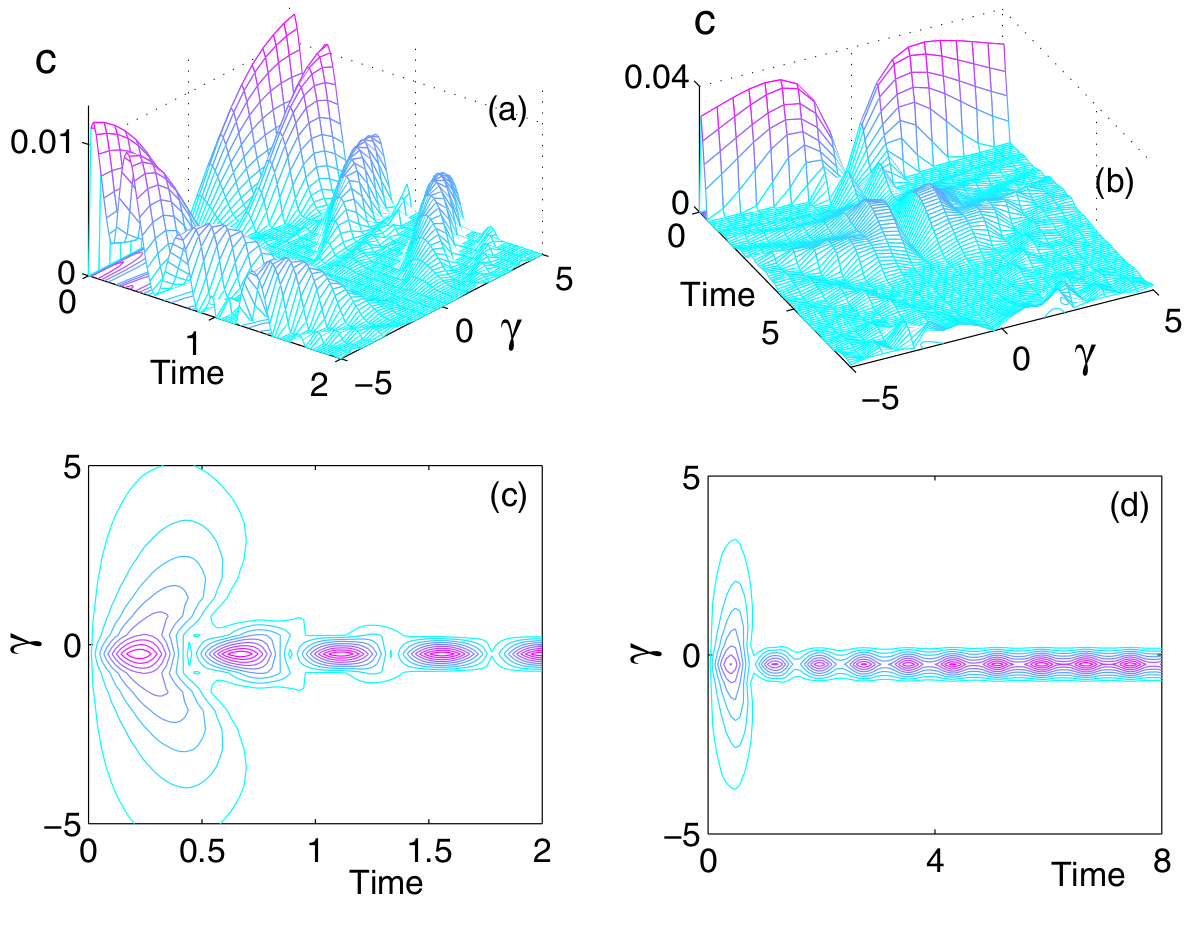
\includegraphics[scale=0.3]{fig1}
	\caption {Совпадение вспомогательных пар частиц как функция времени и параметров анизотропии ~\cite{yi}}
	\label{}
\end{figure}

В любом случае $|\Gamma_{ij;mn}(t)|=1$, что указывает на то, что норма любого элемента приведённой матрицы плотности остаётся неизменной. На рис. 2 показано запутывание вспомогательных частиц вблизи области критичности с $\gamma = 0$ и $\lambda = ± 1$. Запутанность резко меняется по линии $\lambda = ± 1$ на временной плоскости. Это отражение критических явлений при запутывании вспомогательных частиц.

\begin{figure}[htp]
	\centering
	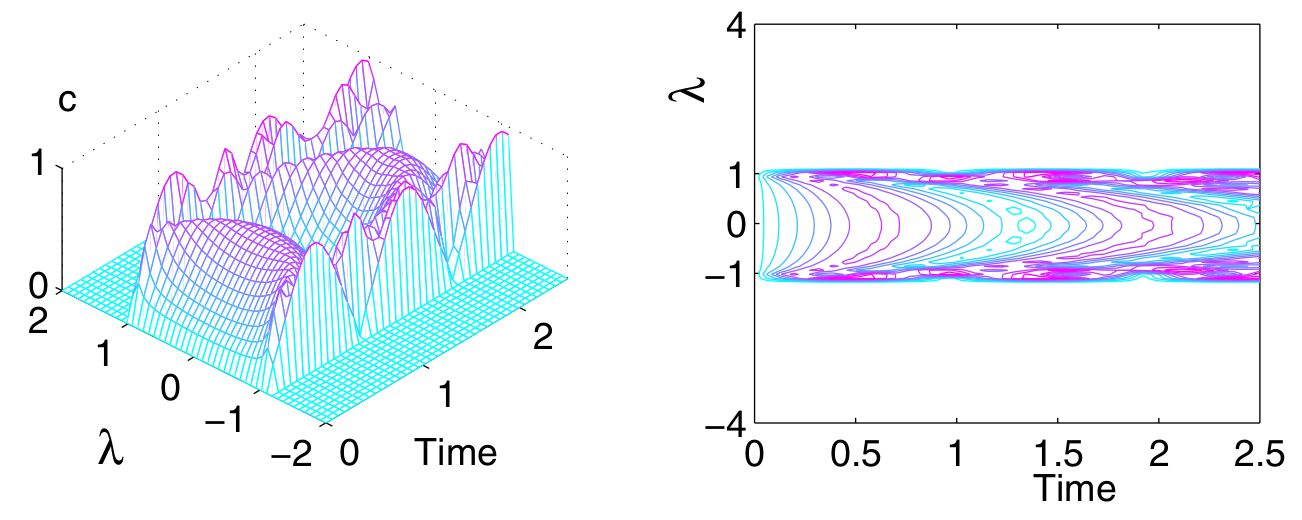
\includegraphics[scale=0.28]{fig2}
	\caption {Согласованность Wootters против времени и $\lambda$ при фиксированном $\gamma=10^{-4}$ ~\cite{yi}}
	\label{}
\end{figure}

Теперь мы переходим к изучению критичности в поперечной модели Изинга. Структура основного состояния поперечной модели кардинально меняется при изменении параметра. Зависимость запутанности от $\lambda$ довольно сложна ~\cite{b2}. Здесь мы представляем анализ для пределов $\lambda → \infty$, $\lambda = 1$ и $\lambda = 0$. В $\lambda → \infty$ пределе основное состояние цепи приближается к произведению спинов, указывающих в положительном направлении $z$. В этом пределе угол смешивания $\Theta_{ij,k}$ и $\Theta_k$ стремится к $-\pi$. Это приводит к $\Gamma_{ij;mn}(t)=1$, что указывает на то, что начальное состояние не эволюционирует со временем, т.е. вспомогательные частицы остаются неразделимыми состояниями. Предел $\lambda = 0$ принципиально отличается от $\lambda → \infty$ предела, поскольку соответствующее основное состояние дважды вырождается при глобальном перевороте спина на $\prod_{l=1}^{N}\sigma_l^z$. Эта симметрия нарушается при $|\lambda |= 1$ и цепочка приобретает ненулевую намагниченность $\langle \sigma^x \rangle \ne 0$ который растёт по мере уменьшения. Это резкое изменение основного состояния спиновой цепи можно найти в запутывании вспомогательных частиц на рис. 3. 

\begin{figure}[htp]
	\centering
	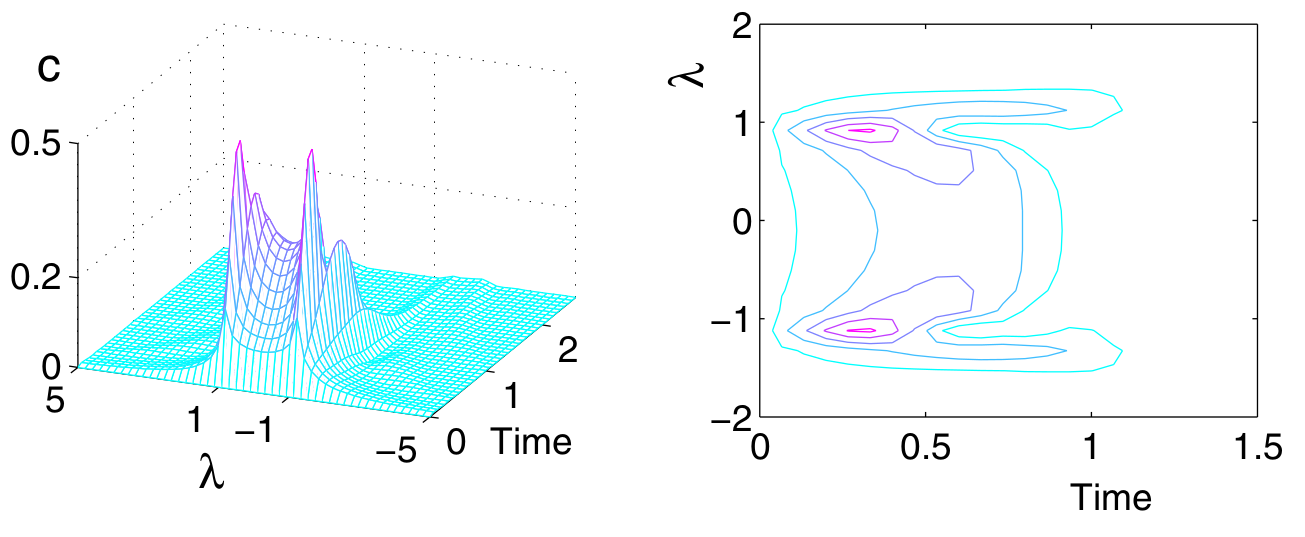
\includegraphics[scale=0.28]{fig3}
	\caption {Запутанность индуцированная поперечной изинговой цепочкой S=1/2, которую можно получить из модели XY, положив $\gamma=1$ ~\cite{yi}}
	\label{}
\end{figure}

На самом деле, основное состояние XY-моделей очень сложно с множеством различных режимов поведения ~\cite{b24,b25}. Как бы то ни было, наблюдается резкое изменение запутанности по линии $|\lambda |= 1$ Рис.4. Это сигнализирует об изменении основного состояния спиновой цепочки с парамагнитной фазы на другие.
Хотя запутанность в обоих случаях с $\gamma = 0$ и $\gamma = 1$ имеет одни и те же свойства вдоль линии $|\lambda|= 1$, т.е. резко меняется в этой критической области. Две вспомогательные частицы никогда не эволюционируют в случае $\gamma = 0$, в то время как две в конечном итоге эволюционируют в состояния указателя в другом случае, кроме $\lambda → \infty$, следовательно, нет запутанности между вспомогательными частицами в более позднем случае при $ t → \infty $ и $ N → \infty$.

Связь между запутанностью во вспомогательных частицах и критичностью спиновой цепочки можно понимать как сингулярность в одном или нескольких $\rho_{ij;mn}(t)$ элементах приведённой матрицы плотности в критических точках. Чтобы показать это, напомним, что

\begin{equation}
\rho_{ij;mn}(t)=\frac{1}{4}\langle\phi_B(0)|e^{-iH_{ij}t}e^{-iH_{kl}t}|\phi_B(0)\rangle
\label{eq_6}
\end{equation}

с теми же обозначениями и начальными состояниями, данными перед уравнением ~\ref{eq_3}. Обратите внимание, что $|\phi_B(0)\rangle$ было взято в качестве основного состояния $|0\rangle$ $H_B$, но оно не является собственным состоянием $H_{ij}$ с $\Lambda_{ij} \ne \lambda$. Разложив $|0\rangle_B$ по собственному состоянию $|\alpha\rangle_B^{ij}$  $H_{ij}$, $\alpha = 0,1,\dots,)$


\begin{equation}
|0\rangle_B=c_0^{ij}|0\rangle_B^{ij} + \sum\limits_{\alpha \ne 0} c_{\alpha}^{ij}|\alpha \rangle_B^{ij}
\label{eq_7}
\end{equation}

легко доказать, что 
$|c_{\alpha \ne 0}^{ij}| \sim h,g$
где $g << 1$ и $h << 1$. Это именно тот случай, который мы рассматриваем, где $|0\rangle_B^{ij}$ обозначает основное состояние $H_{ij}$. Следовательно

\begin{equation}
\rho_{ij;mn}(t) \sim \frac{1}{4}c_0^{ij}[c_0^{kl}]_B^{*kl}
\langle 0|0 \rangle_B^{ij}e^{-i(\Omega_{ij}-\Omega_{kl})t}
\label{eq_8}
\end{equation}

до первого порядка $g$ и $h$. Здесь $\Omega_{ij}$ обозначает энергию основного состояния $H_{ij}$. Как наблюдалось в ~\cite{b26}, внезапное падение в $\langle 0|0 \rangle_B^{ij}$ может сигнализировать об областях критичности в спиновой цепочке. Следовательно, запутанность как функция $\rho_{ij;mn}(t)$ может сигнализировать о критичности цепи.

\begin{figure}[htp]
	\centering
	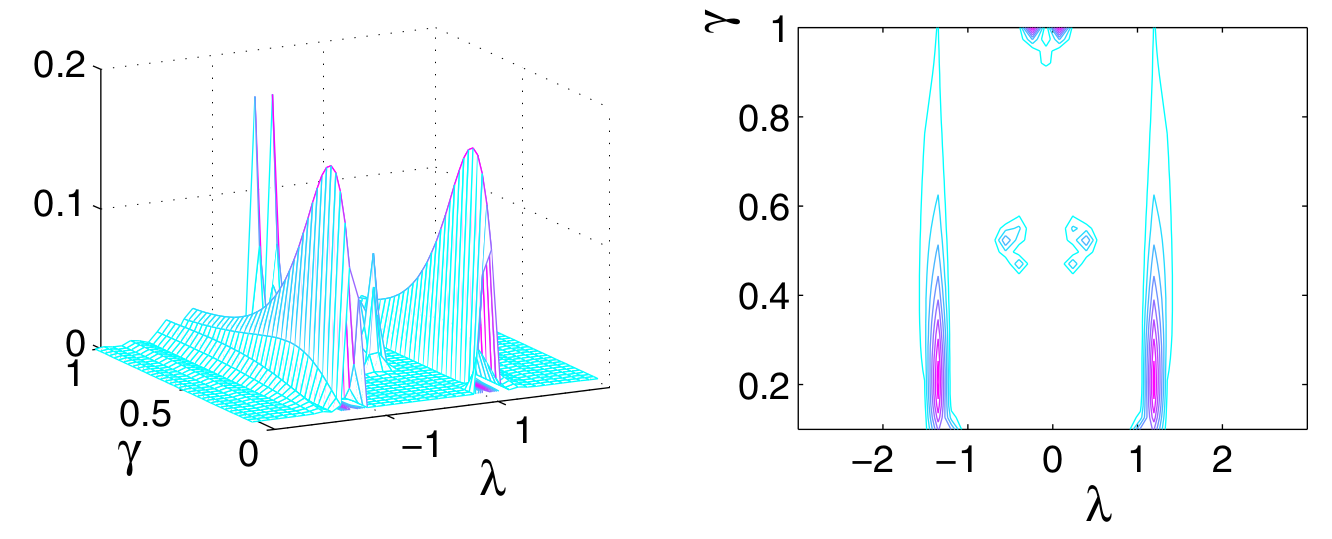
\includegraphics[scale=0.28]{fig4}
	\caption {Согласованность Wootters в момент времени t = 0,75. Положения пиков на оси не меняются со временем ~\cite{yi}}
	\label{}
\end{figure}


Это обсуждение, помимо теоретических интересов, предлагает возможный экспериментальный метод изучения критических явлений без необходимости определения состояния системы, в частности, при наличии вырождения. Модель XY может быть реализована с захваченными ионами под действием нерезонансных волн 19 следующим образом. Рассмотрим систему ловушек, физическая реализация которой соответствует кулоновским цепочкам в ловушках Пеннинга или массиву ионных микроловушек. Кулоновское отталкивание вместе с захваченным потенциалом и движением ионов дает набор коллективных мод колебаний, эти коллективные моды могут быть связаны с внутренними состояниями ионов условными силами. Направления условных сил ~\cite{b19} будут определять эффективные связи между эффективными спинами. Чтобы смоделировать модель XY, мы применим две условные силы в обоих направлениях $x$ и $y$. Эффективное взаимодействие пропорционально $1/r^3$, где $r$ представляет собой относительное расстояние между ионами. Хотя соединения зависят от расстояния, показано, что критические свойства аналогичны идеальным моделям ~\cite{b19,b27}, рассмотренным в этой статье. Связь вспомогательных частиц с цепочкой, которые разделяют другой захват с ионами в цепочке, может быть смоделирована таким же образом, где прикладывается условная сила в одном направлении. Частицы в цепи могут окружать вспомогательные частицы, так что связи вспомогательных частиц с частицами в цепи равны.
Это предложение также может быть реализовано с ультра-холодными атомами в оптической решётке методом, представленным в ~\cite{b28}. Мы хотели бы отметить, что предотвращение любого обмена энергией между цепочкой и вспомогательными частицами может быть сложной задачей в экспериментах. Требование равномерного сцепления также очень сложно экспериментально. Тем не менее, в этой статье установлена связь между запутанностью и критичностью с другой стороны, что может пролить свет на понимание критичности со стороны вспомогательных частиц, и может открыть способ охарактеризовать и экспериментально обнаружить квантовый фазовый переход с точки зрения теории квантовой информации ~\cite{b29}, где рассматриваются две вспомогательные функции, связанные с двумя частицами на разных участках цепи. С помощью этой модели была установлена связь между качеством передачи состояния и спектральным зазором цепи.

\section{Заключение}
Предложенный в ~\cite{b1} метод изучения критических явлений в системах многих тел интересно проверить при других условиях. Было обнаружено, что критичность отражается в запутанности сопряжённых с цепочкой вспомогательных частиц и резко меняется вдоль линии критических точек. Это резкое изменение было объяснено с точки зрения отражения квантовых фазовых переходов, которые приводят к коллективности связей спиновой цепочки с вспомогательные частицы. Также в ~\cite{b30} был сделан вывод, что квантовая критическая система многих тел также может отражать свою критичность в декогеренции квантовой системы, которая с ней взаимодействует - этот факт также интересно проверить при далёких от абсолютного 0 температурах. Проведение этих экспериментов с частицами ионизирующего излучения прольёт свет на роль окружающей среды в обработке квантовой информации, откроют путь для изучения критических явлений в системах многих тел, а также дадут старт практическому созданию квантового компьютера на источниках ионизирующего излучения. Получение и обобщение этих результатов на широкий круг материалов и источников излучения - многообещающий и сложный вопрос, который заслуживает обширного исследования.


\begin{thebibliography}{3}
\bibitem{yi}
Yi, X. X., Cui, H. T., \& Wang, L. C. (2006). Entanglement induced in spin-1∕2particles by a spin chain near its critical points. Physical Review A, 74(5). doi:~\url{10.1103/physreva.74.054102} 

\bibitem{b1}
M.A.Nielsen and I.L.Chuang, Quantum Computation andQuantum Information Cambridge University Press, Cambridge, 2000.

\bibitem{b2}
S. Sachdev,Quantum Phase Transition Cambridge UniversityPress, Cambridge, 1999.

\bibitem{b3}
T. J. Osborne and M. A. Nielsen, Phys. Rev. A66, 032110 -- 2002.

\bibitem{b4}
G. Vidal, J. I. Latorre, E. Rico, and A. Kitaev, Phys. Rev. Lett.90, 227902 -- 2003.

\bibitem{b5}
A. Osterloh, L. Amico, G. Falci, R. Fazio, Nature London 416, 608 -- 2002.

\bibitem{b6}
L. A. Wu, M. S. Sarandy, and D. A. Lidar, Phys. Rev. Lett.93,250404 -- 2004.

\bibitem{b7}
Y. Chen, P. Zanardi, Z. D. Wang, and F. C. Zhang, New J.Phys.8,97 -- 2006; Y. Chen, Z. D. Wang, and F. C. Zhang,Phys. Rev. B73, 224414 -- 2006.

\bibitem{b8}
S. J. Gu, S. S. Deng, Y. Q. Li, and H. Q. Lin, Phys. Rev. Lett.93, 086402 -- 2004.

\bibitem{b9}
F. Verstraete, M. Popp, and J. I. Cirac, Phys. Rev. Lett.92,027901 -- 2004.

\bibitem{b10}
M. B. Plenio, S. F. Huelga, A. Beige, and P. L. Knight, Phys.Rev. A59, 2468 -- 1999; M. B. Plenio and S. F. Huelga, Phys.Rev. Lett.88, 197901, 2002.

\bibitem{b11}
S. Bose, P. L. Knight, M. B. Plenio, and V. Vedral, Phys. Rev.Lett.83, 5158 -- 1999.

\bibitem{b12}
A. Beige, S. Bose, D. Braun, S. F. Huelga, P. L. Knight, M. B.Plenio, and V. Vedral, J. Mod. Opt.47, 2583 -- 2000.

\bibitem{b13}
P. Horodecki, Phys. Rev. A63, 022108 -- 2001.

\bibitem{b14}
D. Braun, Phys. Rev. Lett.89, 277901 -- 2002.

\bibitem{b15}
X. X. Yi, C. S. Yu, L. Zhou, and H. S. Song, Phys. Rev. A68,052304 -- 2003.

\bibitem{b16}
F. Benatti, R. Floreanini, and M. Piani, Phys. Rev. Lett.91,070402 -- 2003

\bibitem{b17}
S. Shresta, C. Anastopoulos, A. Dragulescu, and B. L. Hu,Phys. Rev. A71, 022109 -- 2005.

\bibitem{b18}
L. M. Duan, E. Demler, and M. D. Lukin, Phys. Rev. Lett.91,090402 -- 2003.

\bibitem{b19}
D. Porras and J. I. Cirac, Phys. Rev. Lett.92, 207901 -- 2004;X. L. Deng, D. Porras, and J. I. Cirac, Phys. Rev. A72,063407 -- 2005.

\bibitem{b20}
J. K. Pachos and M. B. Plenio, Phys. Rev. Lett.93, 056402 -- 2004.

\bibitem{b21}
E. Lieb, T. Schultz, and D. Mattis, Ann. Phys.16, 407 -- 1961.

\bibitem{b22}
S. Katsura, Phys. Rev.127, 1508 -- 1962.

\bibitem{b24}
E. Barouch and B. M. McCoy, Phys. Rev. A2, 1075 -- 1970;3, 786 -- 1971.

\bibitem{b25}
M. F. Yang, Phys. Rev. A71, 030302R -- 2005.

\bibitem{b26}
P. Zanardi and N. Paunkovic, Phys. Rev. E74, 031123 -- 2006.

\bibitem{b27}
A. Dutta and J. K. Bhattacharjee, Phys. Rev. B64, 184106 -- 2001.

\bibitem{b28}
Angelo C. M. Carollo and Jiannis K. Pachos, Phys. Rev. Lett.95, 157203 -- 2005.

\bibitem{b29}
M. J. Hartmann, M. E. Reuter, and M. B. Plenio, New J. Phys.8,94 -- 2006.

\bibitem{b30}
H. T. Quan, Z. Song, X. F. Liu, P. Zanardi, and C. P. Sun, Phys.Rev. Lett.96, 140604 -- 2006

\end{thebibliography}

\end{document}